\documentclass[conference]{IEEEtran}
\IEEEoverridecommandlockouts

% ---------------- Preamble ----------------
\usepackage{cite}
\usepackage{amsmath,amssymb,amsfonts}
\usepackage{graphicx}
\usepackage{textcomp}
\usepackage{xcolor}
\usepackage{url}
\usepackage{booktabs}
\usepackage{array}
\usepackage{tabularx}
\usepackage{tikz}
\usetikzlibrary{arrows.meta,positioning,shapes.geometric}

\graphicspath{{figures/}}

\begin{document}

\title{Disagreement-Triggered Multi-Agent LLM Deliberation for Retail Demand Forecasting and
Restocking Decisions}

% Replace the placeholders below (one \IEEEauthorblockN/\IEEEauthorblockA pair per author).
\author{
\IEEEauthorblockN{[Author Name]}
\IEEEauthorblockA{\textit{Dept. of CSE (AI/ML)} \\
\textit{Dayananda Sagar University}\\
Bengaluru South, India \\
[email]}
\and
\IEEEauthorblockN{[Supervisor Name]}
\IEEEauthorblockA{\textit{Dept. of CSE (AI/ML)} \\
\textit{Dayananda Sagar University}\\
Bengaluru South, India \\
[email]}
}

\maketitle

% =====================================================================
\begin{abstract}
Calling a large language model (LLM) on every retail demand forecast is costly, and a natural
shortcut is to call it only when specialised forecasting agents disagree. This paper tests that
idea under a frozen protocol. In the proposed system, RetailSense, a LightGBM Historical agent and
Calendar, Weather and Trend agents forecast daily item demand; a confidence-weighted disagreement
score $D$ triggers an LLM critic and one bounded revision round when $D$ reaches a threshold frozen
on validation data. Code, never the LLM, computes the final forecast and the order quantity, and
every system is evaluated through the same $(s,S)$ inventory simulator. One locked test run per
dataset covers a simulated Mumbai grocery store with logged demand drivers and real daily sales from
the Czech online grocer Rohlik. On the test splits, disagreement is a weak but significant risk
signal (Spearman $\rho=0.072$ on simulated India, $0.119$ on real Rohlik). Selective deliberation does
not improve accuracy: it is statistically equivalent to always-on deliberation, to random triggering
and to no deliberation within 1\% of WAPE. Its only demonstrated benefit is 73--83\% fewer LLM calls
at that equivalent accuracy. Stronger single models beat every multi-agent variant: LightGBM on India
(test WAPE 0.369 vs 0.378) and ETS on Rohlik (0.150 vs 0.175). Post-hoc validation analyses show that the failure is not an artefact of correlated agents
or of a weak critic: independent agents do not make $D$ a better warning, and a 31B critic that acts
on the true demand driver still gains nothing from selection by $D$.
\end{abstract}

\begin{IEEEkeywords}
demand forecasting, multi-agent systems, large language models, forecast disagreement, selective
deliberation, equivalence testing, inventory control
\end{IEEEkeywords}

% =====================================================================
\section{Introduction}

A store manager who restocks shelves every week must decide how much of each item to order before
demand is known. Ordering too little loses sales; ordering too much ties up cash and shelf space.
The forecast behind that decision draws on several kinds of evidence: recent sales, the calendar,
the weather and shifts in customer interest. Gradient-boosted models such as LightGBM~\cite{ke2017}
combine these signals well and dominated the M5 retail benchmark~\cite{makridakis2022}. Large
language models may add a different ability, reasoning about conflicting evidence and which source
to trust~\cite{du2024}, but each call costs time and money, and the value of an LLM in numeric
forecasting is contested~\cite{tan2024}.

This paper asks whether an LLM can be used \emph{selectively}, only on the forecasts where it is most
likely to help. The idea comes from forecast combination: combined forecasts usually beat single
ones~\cite{bates1969,timmermann2006,wang2023}, and the spread between forecasters signals
uncertainty, although imperfectly~\cite{zarnowitz1987,whitaker1998}. If agents disagree, the case may
be risky and worth a closer look.

\subsection{Research Objectives}
The research question is: \emph{does disagreement-triggered deliberation among heterogeneous
forecasting agents improve demand forecasts and restocking decisions compared with statistical
forecasting, a single model, simple consensus and always-on deliberation?} It is split into five
hypotheses: \textbf{H1} disagreement $D$ is positively associated with forecast error; \textbf{H2}
deliberation lowers error on the triggered cases; \textbf{H3} selective deliberation matches always-on
deliberation at a fraction of the LLM cost; \textbf{H4} $D$ is a better trigger than chance;
\textbf{H5} better forecasts give better inventory outcomes. H4 is the central test: if a random
trigger at the same rate does as well, $D$ adds nothing.

\subsection{Contributions}
\begin{itemize}
\item A \textbf{frozen evaluation protocol} for selective LLM use: the threshold $\tau$ and the
prompt are frozen on validation before one locked test run per dataset, a random trigger at the
same rate isolates the value of $D$, and ``no difference'' claims rest on equivalence
tests~\cite{schuirmann1987} and minimum detectable effects.
\item A \textbf{simulator with logged ground-truth drivers}, built on real weather~\cite{openmeteo}
and a real festival calendar, which makes it possible to check whether the critic identifies the
evidence that actually moved demand.
\item A \textbf{diagnosis} that varies agent design, critic size and trigger, and scores each against
the frozen systems on the same cases.
\item A \textbf{real-data replication} on Rohlik sales~\cite{rohlik} with ETS, LightGBM and the
Chronos foundation model~\cite{ansari2024} as baselines.
\end{itemize}

Section~II reviews the literature, Section~III describes the methodology, Section~IV reports the
findings, Section~V discusses them and Section~VI concludes.

% =====================================================================
\section{Literature Review}\label{sec:related}

\begin{table*}[!t]
\centering
\caption{Literature Survey: Prior Work, Limitations and the Gap Addressed by RetailSense}
\label{tab:literature}
\footnotesize
\renewcommand{\arraystretch}{1.15}
\begin{tabularx}{\textwidth}{|c|p{2.2cm}|p{2.6cm}|X|X|X|}
\hline
\textbf{\#} & \textbf{Reference} & \textbf{Method} & \textbf{Key Contribution} &
\textbf{Limitation / Gap} & \textbf{How This Work Responds} \\
\hline
1 & Bates \& Granger~\cite{bates1969}; Wang \emph{et al.}~\cite{wang2023} & Forecast combination &
Weighted combinations beat their inputs on average & Combination weights only; no rule for when to
look closer at a case & Confidence-weighted consensus plus a disagreement-based trigger \\
\hline
2 & Zarnowitz \& Lambros~\cite{zarnowitz1987}; Whitaker \& Loughe~\cite{whitaker1998} &
Disagreement / ensemble spread & Spread correlates with uncertainty & Spread understates
uncertainty; spread--skill link can be weak & Tests $D$ against error and against a random trigger \\
\hline
3 & Makridakis \emph{et al.}~\cite{makridakis2022} & M5 competition, LightGBM & Gradient boosting
wins retail forecasting & Accuracy only; no inventory decision & Every system scored through one
$(s,S)$ simulator \\
\hline
4 & Du \emph{et al.}~\cite{du2024}; Madaan \emph{et al.}~\cite{madaan2023} & Multi-agent debate;
Self-Refine & Critique and revision improve LLM answers & Applied to text tasks; LLM writes the
answer & LLM only re-weights numeric agents inside bounds \\
\hline
5 & Huang \emph{et al.}~\cite{huang2024}; Sharma \emph{et al.}~\cite{sharma2024} & Self-correction;
sycophancy & LLMs often fail to self-correct and yield to pressure & Risk that ``deliberation''
measures compliance & Hold-rate gate; holding is a normal answer \\
\hline
6 & Chen \emph{et al.}~\cite{chen2023}; Ong \emph{et al.}~\cite{ong2025} & FrugalGPT; RouteLLM &
Cascades and learned routers cut LLM cost & Routers are rarely compared with a random router at the
same rate & Random and learned triggers as controls \\
\hline
7 & Gruver \emph{et al.}~\cite{gruver2023}; Tan \emph{et al.}~\cite{tan2024} & LLMs as forecasters &
Zero-shot numeric forecasting & Removing the LLM often does not hurt accuracy & LLM never produces
the demand number \\
\hline
8 & Ansari \emph{et al.}~\cite{ansari2024} & Chronos foundation model & Zero-shot forecasts of unseen
series & Not designed for decisions or for explaining conflicts & Used as a strong baseline \\
\hline
9 & Yang \emph{et al.}~\cite{yang2025} & Transformer + hierarchical multi-agent RL & Joint forecasting
and inventory, lower MAPE and stockouts & Agents split by supply-chain level; zero-filled missing
sales; single estimates & Agents split by evidence source; missing kept missing; frozen protocol \\
\hline
\end{tabularx}
\end{table*}

Table~\ref{tab:literature} summarises the work this study builds on.

\subsection{Forecast Combination and Disagreement}
Bates and Granger~\cite{bates1969} showed that a combination weighted by past error can beat each of
its inputs, and Timmermann~\cite{timmermann2006} explains why combinations tend to win, especially
when information sets cannot be pooled into one model. Disagreement between forecasters correlates
with uncertainty but understates it~\cite{zarnowitz1987}, and even for a perfect weather ensemble the
spread--skill relationship can be modest~\cite{whitaker1998}. RetailSense uses both ideas: a
confidence-weighted combination on the fast path, and the spread around it as a trigger.

\subsection{LLM Deliberation and Its Failure Modes}
Multi-agent debate is reported to improve reasoning and factuality~\cite{du2024}, and Self-Refine
improves outputs through a critique-then-revise loop~\cite{madaan2023}. Without external feedback,
however, LLM self-correction often fails~\cite{huang2024}, and assistants trained with human feedback
tend to change answers under social pressure~\cite{sharma2024}. RetailSense therefore confines the
LLM to bounded re-weighting and tracks how often each agent keeps its position.

\subsection{Selective and Cost-Aware LLM Use}
FrugalGPT studies LLM cascades~\cite{chen2023}, and RouteLLM learns per-query routers~\cite{ong2025}.
Triggering on $D\ge\tau$ is a simple, unlearned router; this study evaluates it against a random
router at the same rate and against a learned one.

\subsection{Forecasting Models and Inventory}
LLMs can forecast numeric series zero-shot~\cite{gruver2023} or be reprogrammed as
forecasters~\cite{jin2024}, yet ablations show that the LLM component often adds
little~\cite{tan2024}; pretrained foundation models such as Chronos~\cite{ansari2024} are now a
standard baseline. Forecast accuracy does not translate directly into inventory
performance~\cite{syntetos2010,kourentzes2020}. The closest system, MARIOD~\cite{yang2025}, couples a
transformer forecaster with multi-agent reinforcement learning for ordering. It is the research
reference and motivation for this work, not a numerical baseline: it was not reimplemented, and no
claim is made that RetailSense outperforms it. The gap addressed here
is a controlled test of \emph{when} an LLM should be consulted, with the decision left to a
transparent $(s,S)$ policy~\cite{silver2017}.

% =====================================================================
\section{Methodology}\label{sec:method}

\subsection{System Overview}
Fig.~\ref{fig:system} shows the pipeline. Each agent sees one kind of evidence; the orchestrator
computes $D$; if $D<\tau$ the confidence-weighted consensus is returned, otherwise an LLM critic
explains the conflict and each agent gets one bounded revision. The final forecast feeds an $(s,S)$
policy that outputs RESTOCK, HOLD or REDUCE.

\begin{figure}[t]
\centering
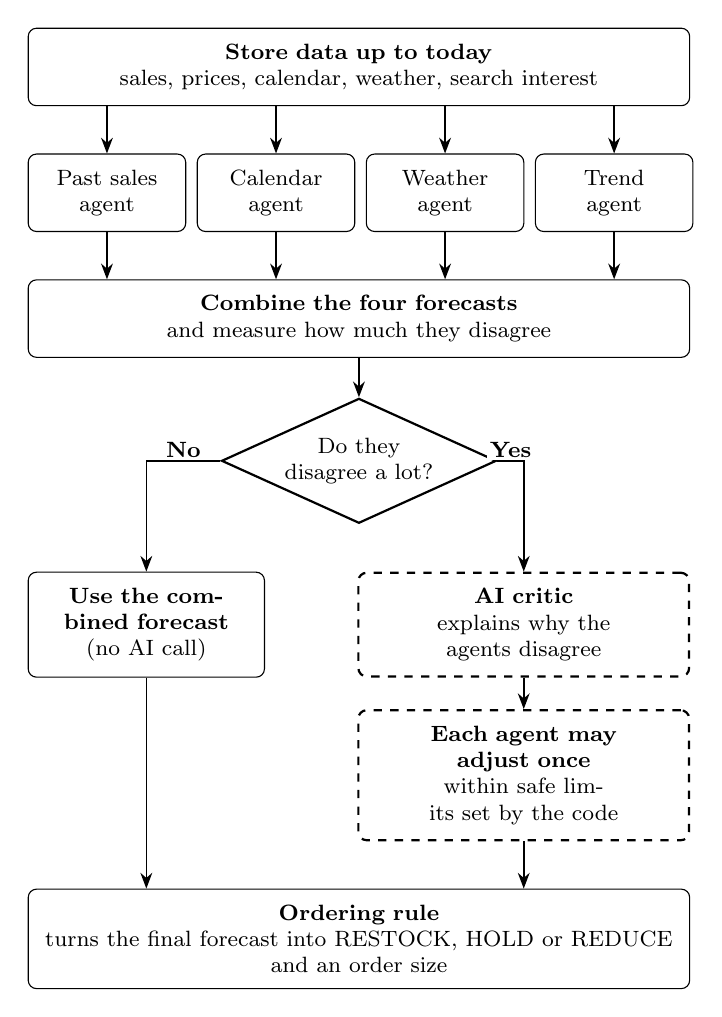
\begin{tikzpicture}[font=\footnotesize,
  box/.style={draw, rounded corners=3pt, align=center, inner sep=2mm, minimum height=8mm},
  ai/.style={box, dashed, thick},
  arr/.style={-{Stealth[length=2mm]}, semithick},
  lab/.style={font=\footnotesize\bfseries, fill=white, inner sep=1pt}]

\node[box, text width=80mm] (data) {\textbf{Store data up to today}\\
  sales, prices, calendar, weather, search interest};

\node[box, text width=16mm, anchor=north west] (a1) at ([yshift=-6mm]data.south west)
  {Past sales\\agent};
\node[box, text width=16mm, right=1.33mm of a1] (a2) {Calendar\\agent};
\node[box, text width=16mm, right=1.33mm of a2] (a3) {Weather\\agent};
\node[box, text width=16mm, right=1.33mm of a3] (a4) {Trend\\agent};

\node[box, text width=80mm, anchor=north west] (comb) at ([yshift=-6mm]a1.south west)
  {\textbf{Combine the four forecasts}\\ and measure how much they disagree};

\node[draw, diamond, aspect=2.2, align=center, inner sep=0.5mm, thick,
      below=5mm of comb] (dia) {Do they\\ disagree a lot?};

\node[box, text width=26mm, anchor=north west] (fast) at ([yshift=-6mm]comb.south west |- dia.south)
  {\textbf{Use the combined forecast}\\ (no AI call)};
\node[ai, text width=38mm, anchor=north east] (crit) at ([yshift=-6mm]comb.south east |- dia.south)
  {\textbf{AI critic}\\ explains why the agents disagree};
\node[ai, text width=38mm, below=4mm of crit] (rev)
  {\textbf{Each agent may adjust once}\\ within safe limits set by the code};

\node[box, text width=80mm, anchor=north] (order) at ([yshift=-6mm]comb.south |- rev.south)
  {\textbf{Ordering rule}\\ turns the final forecast into RESTOCK, HOLD or REDUCE\\ and an order
  size};

\foreach \a in {a1,a2,a3,a4} {
  \draw[arr] (data.south -| \a.north) -- (\a.north);
  \draw[arr] (\a.south) -- (\a.south |- comb.north);
}
\draw[arr] (comb) -- (dia);
\draw[arr] (dia.west) -| node[lab, pos=0.25, above]{No} (fast.north);
\draw[arr] (dia.east) -| node[lab, pos=0.25, above]{Yes} (crit.north);
\draw[arr] (crit) -- (rev);
\draw[arr] (fast.south) -- (fast.south |- order.north);
\draw[arr] (rev.south) -- (rev.south |- order.north);
\end{tikzpicture}
\caption{How RetailSense works. Four agents each forecast demand from one kind of information. If
they mostly agree, their combined forecast is used straight away. If they disagree a lot, an AI
critic explains the conflict and each agent may adjust its forecast once, within limits set by the
code. A fixed ordering rule, not the AI, decides how much to order. Dashed boxes are AI steps.}
\label{fig:system}
\end{figure}

\subsection{Datasets and Splits}
\emph{India (simulated):} store MUM\_1 with 60 items, generated with a fixed seed from real
Open-Meteo weather for Mumbai~\cite{openmeteo} and a real festival calendar. Demand is a product of
base level, weekday, growth, weather, festival, payday, promotion and interest-shock multipliers with
gamma-Poisson noise and stock-outs, and every multiplier is logged. \emph{Rohlik (real):} the Kaggle
Rohlik Sales Forecasting Challenge v2~\cite{rohlik}, warehouse Prague\_1, top 60 items with a complete
record; there is no search-interest data, so the Trend agent is omitted. The splits are chronological:
India train d\_1--1799 (5 Jan 2019 -- 8 Dec 2023), validation d\_1800--1885, test d\_1886--1941
(4 Mar -- 28 Apr 2024); Rohlik train d\_1--1260 (1 Aug 2020 -- 12 Jan 2024), validation
d\_1261--1346, test d\_1347--1402 (8 Apr -- 2 Jun 2024). Models are fitted on train, every design decision and $\tau$ use
validation, and each test split is read once. Every feature row carries an \texttt{available\_at}
date, and tests assert that it never follows the prediction time; missing sales stay missing.

\subsection{Forecasting Agents}
Each agent returns a schema-validated forecast for horizons $h=1,\dots,7$, a 10--90\% band and a
confidence; an invalid or abstaining agent is excluded and flagged, never converted to a zero. The
\emph{Historical agent} is LightGBM with a Tweedie objective plus two quantile models, trained on
lagged sales (lags $h$, 7, 14, 28; rolling statistics over 7, 28 and 56 days), price and item
identity, with one direct model per horizon. The \emph{Calendar, Weather and Trend agents} are
residual adjusters: each forecasts $b+g_i(b,x_i)$, where $b$ is the baseline and $g_i$ a LightGBM
model trained on out-of-fold residuals from five expanding time folds using only its own evidence
$x_i$. Confidence is $c_i=1/(1+\mathrm{WAPE}_i)$ over the trailing 28 revealed days.

\subsection{Disagreement Score and Trigger}
At $h=1$, with $w_i=c_i/\sum_j c_j$ and $\bar y=\sum_i w_i y_i$,
\begin{equation}
D=\frac{\sqrt{\sum_i w_i\,(y_i-\bar y)^2}}{\max(\bar y,1)},
\end{equation}
a confidence-weighted coefficient of variation that is scale-invariant and zero when all forecasts
agree (both unit-tested). The threshold $\tau$ is the 80th percentile of validation $D$, written into
the configuration before any test data are read ($\tau=0.0769$ India, $0.0654$ Rohlik).

\subsection{LLM Critic and Bounded Revision}
Deliberation is one round in a LangGraph state machine using Llama~3.1~8B~\cite{llama3} at
temperature 0. The critic receives each agent's forecast, band, confidence and evidence plus 14 days
of revealed sales, and returns a JSON report with no numeric field: the main conflict, a
strong/moderate/weak rating of each agent's evidence and one question per agent. Each revision
returns a multiplier $m_i$ and a revised value $y'_i$; holding position is a normal answer. Code
clips $m_i$ to $[0.25,2.0]$ and $y'_i$ to the agent's band and computes
$\hat y=\sum_i w'_i y'_i$ with $w'_i\propto c_i m_i$. Invalid output gets one retry, then falls back
to the fast path.

\subsection{Inventory Policy}
A periodic-review $(s,S)$ policy~\cite{silver2017} uses lead time $L=3$, review period $R=7$,
$z=1.65$ and case pack 6, with $\sigma_h=(u_h-l_h)/2.563$ from the band,
\begin{equation}
s=\sum_{h\le L} f_h + z\sqrt{\textstyle\sum_{h\le L}\sigma_h^2},\quad
S=\sum_{h\le L+R} f_h + z\sqrt{\textstyle\sum_{h\le L+R}\sigma_h^2},
\end{equation}
ordering $S-\mathrm{IP}$ in whole case packs when the inventory position $\mathrm{IP}\le s$
(RESTOCK); otherwise HOLD, or REDUCE when $\mathrm{IP}$ exceeds $S$ plus one week of forecast demand.
REDUCE is an advisory overstock flag only: it orders zero and the simulator has no returns or
markdowns, so it affects stock and cost exactly as HOLD does. Holding
cost is 25\% of price per year, order cost \$5 and lost-sales cost one unit price. A test asserts
that the inventory code cannot import the LLM layer.

\subsection{Baselines and Evaluation}
Nine systems are compared: seasonal naive, ETS, LightGBM with all features, the Historical agent, the
simple and confidence-weighted multi-agent consensus, a random trigger at the same rate, always-on
deliberation and RetailSense. WAPE is the primary metric. H1 uses Spearman's $\rho$ between $D$ and
relative error and the AUROC of $D$ for the worst 20\% of errors. Comparisons use Diebold--Mariano
tests~\cite{diebold1995} with the Harvey--Leybourne--Newbold correction and a paired item bootstrap;
equivalence uses the two one-sided tests procedure~\cite{schuirmann1987} at margins of 0.5\%, 1\% and
2\% of WAPE; H2 is retested with an item-clustered bootstrap; and Holm's procedure~\cite{holm1979}
corrects the confirmatory family. Post-hoc analyses (Section~IV-E) use validation data only, and the
frozen outputs were verified unchanged by checksum.

% =====================================================================
\section{Results and Findings}\label{sec:results}

\subsection{Forecast Accuracy and Inventory Cost}
Table~\ref{tab:results} summarises both test splits. On India the single all-features LightGBM is the
most accurate system (0.3688 against 0.3775 for RetailSense, DM $p=0.003$, Holm-adjusted 0.023) and
wins all three backtest windows. On Rohlik, ETS is the most accurate (Holm-adjusted $p=0.005$). All
multi-agent systems (5--9) lie within 0.0005 WAPE of each other. The cost ranking differs from the
accuracy ranking: ETS is cheapest on India (\$138,621 against \$206,313) and LightGBM on Rohlik
(\$133,467 against \$287,344), so H5 is not supported.

\begin{table*}[t]
\caption{Test Results: $h=1$ WAPE With 95\% Bootstrap CI, Pooled $h=1$--7 WAPE and Total Simulated
Inventory Cost. Best Value per Column in Bold.}
\label{tab:results}
\centering
\scriptsize
\setlength{\tabcolsep}{4pt}
\begin{tabular}{@{}rl ccr ccr@{}}
\toprule
 & & \multicolumn{3}{c}{India (simulated)} & \multicolumn{3}{c}{Rohlik (real)} \\
\cmidrule(lr){3-5}\cmidrule(l){6-8}
\# & System & $h=1$ WAPE [95\% CI] & $h=1$--7 & Cost (\$) & $h=1$ WAPE [95\% CI] & $h=1$--7 & Cost (\$) \\
\midrule
1 & Seasonal naive          & 0.5530 [0.5261, 0.5860] & 0.5488 & 199,786 & 0.2582 [0.1857, 0.3383] & 0.2522 & 509,438 \\
2 & ETS                     & 0.3904 [0.3712, 0.4121] & 0.4030 & \textbf{138,621} & \textbf{0.1504} [0.1308, 0.1736] & 0.1892 & 262,890 \\
3 & LightGBM, all features  & \textbf{0.3688} [0.3555, 0.3835] & \textbf{0.3782} & 183,250 & 0.1665 [0.1376, 0.1959] & \textbf{0.1858} & \textbf{133,467} \\
4 & Historical agent        & 0.3793 [0.3664, 0.3954] & 0.3902 & 232,910 & 0.1760 [0.1463, 0.2043] & 0.1975 & 314,936 \\
5 & Multi-agent mean        & 0.3778 [0.3646, 0.3931] & 0.3886 & 203,357 & -- & -- & -- \\
6 & Multi-agent, confidence & 0.3777 [0.3646, 0.3931] & 0.3885 & 205,862 & 0.1746 [0.1502, 0.1974] & 0.1993 & 287,802 \\
7 & Random trigger          & 0.3778 [0.3647, 0.3931] & 0.3885 & 206,393 & 0.1747 [0.1509, 0.1971] & 0.1993 & 289,319 \\
8 & Always-on deliberation  & 0.3773 [0.3645, 0.3926] & 0.3884 & 199,868 & 0.1741 [0.1505, 0.1961] & 0.1994 & 278,104 \\
9 & RetailSense             & 0.3775 [0.3643, 0.3929] & 0.3885 & 206,313 & 0.1745 [0.1504, 0.1970] & 0.1993 & 287,344 \\
\bottomrule
\end{tabular}
\end{table*}

\subsection{H1: Disagreement and Error}
$D$ is weakly but significantly associated with error: Spearman $\rho=0.072$ [0.039, 0.108] and AUROC
0.539 on India, $\rho=0.119$ [0.063, 0.176] and AUROC 0.579 on Rohlik (Fig.~\ref{fig:deciles}), both
with Holm-adjusted $p<0.001$. On validation, $D$ adds almost nothing beyond the Historical band width
and item volume as a predictor of large errors. H1 is weakly supported.

\begin{figure*}[t]
\centering
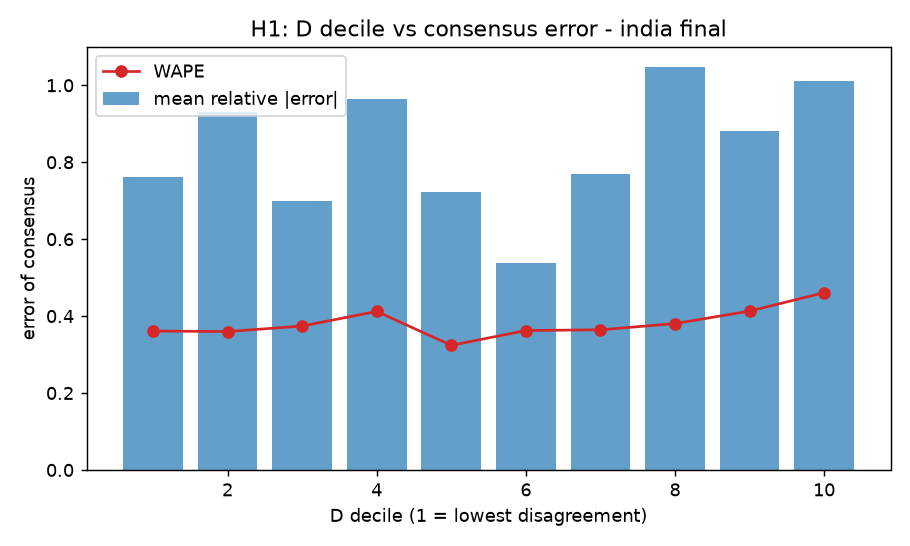
\includegraphics[width=0.49\textwidth]{india_h1_deciles.png}\hfill
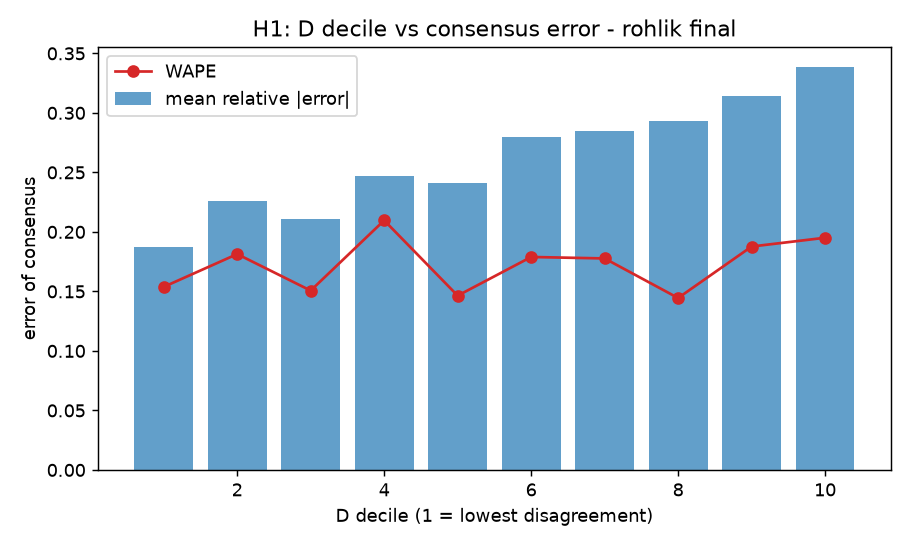
\includegraphics[width=0.49\textwidth]{rohlik_h1_deciles.png}
\caption{Consensus error by decile of disagreement $D$ on the India (left) and Rohlik (right) test
splits. Bars: mean relative absolute error; line: WAPE. The rise with $D$ is weak and non-monotone on
India and clearer on Rohlik.}
\label{fig:deciles}
\end{figure*}

\subsection{H2: Effect on Triggered Cases}
On India, 30.3\% of the 892 triggered test cases improved and 24.6\% worsened. With cases clustered by
item, the mean gain is 0.027 units [0.003, 0.052] (Holm-adjusted $p=0.044$), about 0.2\% of the mean
absolute error, and it did not appear on either validation split or on the Rohlik test split
(clustered $p=0.59$). Agents kept their position in 58.7\% (India) and 53.3\% (Rohlik) of revisions,
so the result is not explained by compliance.

\subsection{H3 and H4: Cost and the Value of the Trigger}
Table~\ref{tab:equiv} shows that selective deliberation is equivalent to always-on deliberation, to
random triggering and to no deliberation within 0.5\% of WAPE on India and within 1\% on Rohlik. The
minimum detectable effects (0.0004--0.0022 WAPE) show that the tests had power to detect differences
of 0.1--1.3\% of WAPE. Selective deliberation uses 1,331 instead of 5,018 LLM calls per 1,000
forecasts on India ($-73\%$) and 696 instead of 4,051 on Rohlik ($-83\%$), so H3 is supported. H4 is
not (DM $p=0.08$ and $0.57$), and along the cost--accuracy curve (Fig.~\ref{fig:costacc}) selective
triggering stays inside the random band.

\begin{table}[t]
\caption{Equivalence on the Test Splits: $h=1$ WAPE Difference With 90\% Item-Bootstrap CI and
Minimum Detectable Effect (80\% Power)}
\label{tab:equiv}
\centering
\scriptsize
\setlength{\tabcolsep}{3pt}
\begin{tabular}{@{}lccc@{}}
\toprule
Comparison & Diff [90\% CI] & MDE & Equiv. at \\
\midrule
\multicolumn{4}{@{}l}{\emph{India}} \\
Selective -- always-on & $+0.0002$ [$-0.0003$, $0.0007$] & 0.0008 & 0.5\% \\
Selective -- random    & $-0.0003$ [$-0.0005$, $-0.0000$] & 0.0004 & 0.5\% \\
Always-on -- none      & $-0.0004$ [$-0.0009$, $0.0001$] & 0.0009 & 0.5\% \\
\midrule
\multicolumn{4}{@{}l}{\emph{Rohlik}} \\
Selective -- always-on & $+0.0004$ [$-0.0009$, $0.0016$] & 0.0021 & 1\% \\
Selective -- random    & $-0.0002$ [$-0.0009$, $0.0004$] & 0.0012 & 1\% \\
Always-on -- none      & $-0.0005$ [$-0.0017$, $0.0009$] & 0.0022 & 1\% \\
\bottomrule
\end{tabular}
\end{table}

\begin{figure*}[t]
\centering
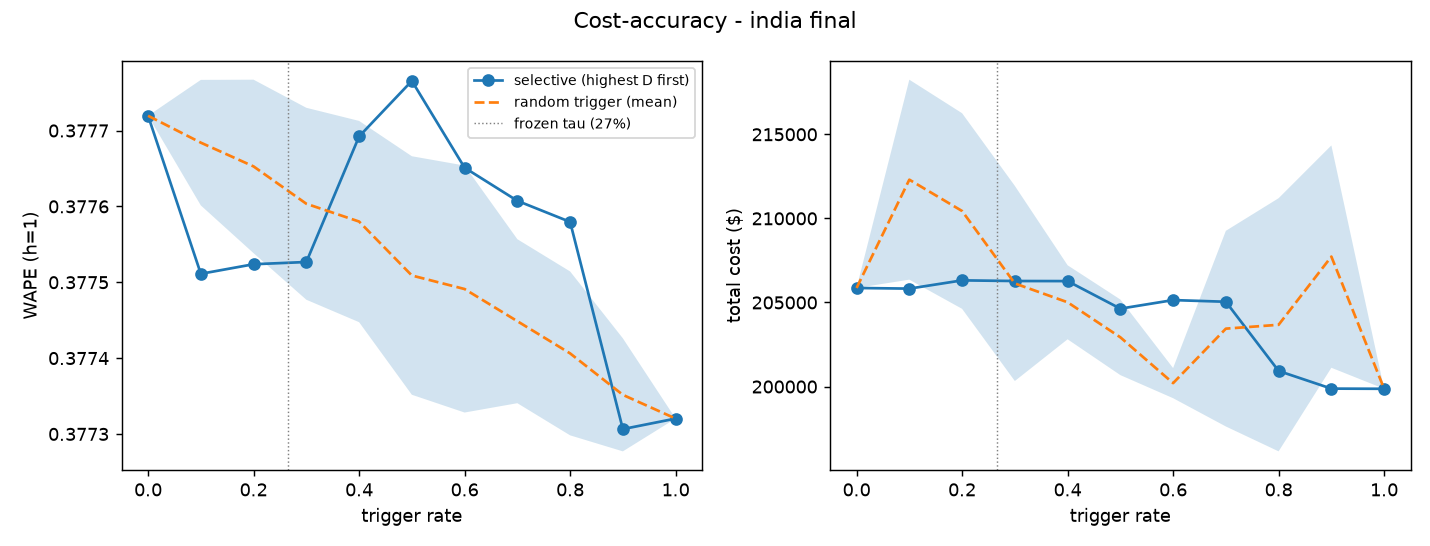
\includegraphics[width=0.49\textwidth]{india_cost_accuracy.png}\hfill
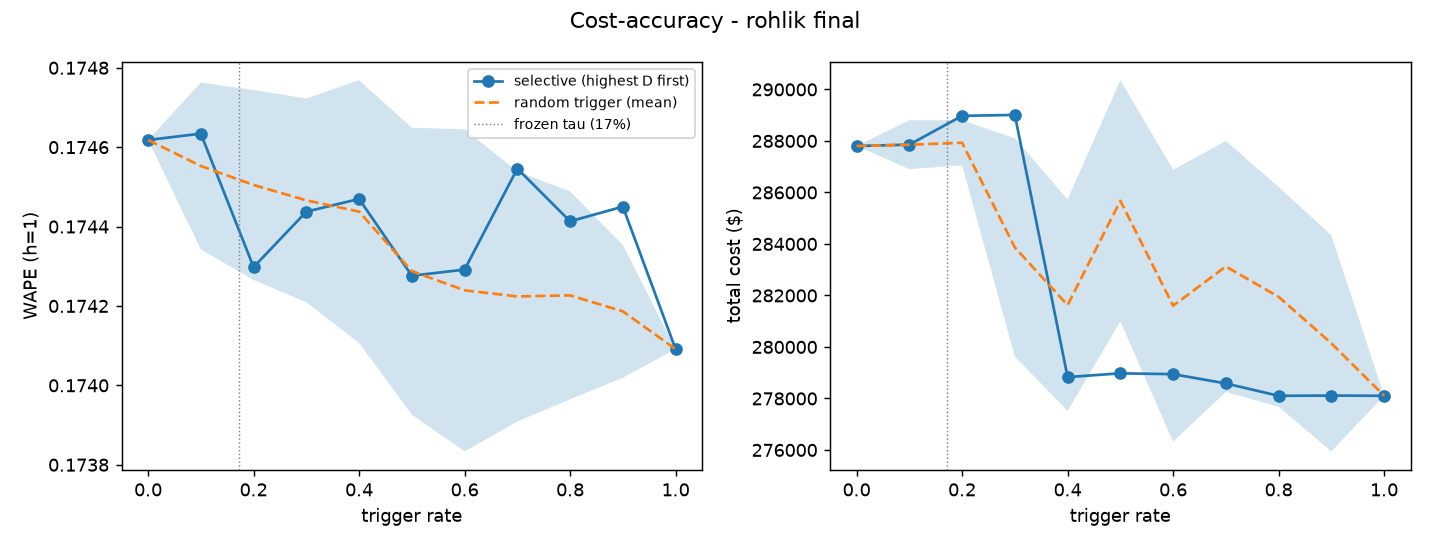
\includegraphics[width=0.49\textwidth]{rohlik_cost_accuracy.png}
\caption{Cost--accuracy curves on the India (left) and Rohlik (right) test splits: $h=1$ WAPE and
total inventory cost as the share of deliberated cases rises, for selective triggering (highest $D$
first) and random triggering (mean and band). The dotted line marks the frozen $\tau$.}
\label{fig:costacc}
\end{figure*}

\subsection{Diagnosis: Why Selective Deliberation Fails}
Four declared post-hoc analyses on validation data test the obvious explanations
(Table~\ref{tab:diagnosis}).

\emph{Correlated agents.} The frozen agents share a baseline (within-item forecast correlation
0.76--1.00), so $D$ could be noise by construction. \emph{Independent} agents that forecast from item
identity and their own evidence only, with no sales history, have within-item correlation near zero.
On Rohlik their $D$ predicts the consensus error better (AUROC 0.667), but only because the
consensus now contains much weaker agents; as a warning for large errors of the strong Historical
forecast, $D$ adds at most 0.013 AUROC in every design.

\emph{Critic quality.} Because the simulator logs every demand multiplier, each India case has a
known true driver. The 8B critic rated the driver's agent ``strong'' 8.3 points more often than other
agents [5.2, 11.7], yet the revisions gave it the same weight as the others. A 31B critic (Gemma~4)
did move weight toward the driver ($+0.088$ [0.017, 0.153]) and lowered always-on WAPE on India,
but with either critic, selection by $D$ was no better than random. The only large deliberation gain
(independent agents with the 31B critic on Rohlik, 64\% of triggered cases improved) repairs errors
those agents introduce and stays worse than the frozen consensus on the same cases.

\emph{No critic.} With the critic removed (agents see each other's forecasts instead, 300 validation
cases), agents held their position in 99\% of revisions and WAPE did not change significantly (India
$-0.0001$, Rohlik $-0.0051$, both CIs include 0). The critic causes almost all revisions, but
they improve about as many cases as they worsen.

\emph{Learned trigger.} A trigger trained to predict the deliberation gain from $D$, its range, band
width and volume was no better than random ($\rho=0.023$ and $-0.022$ with the realised gain),
although a perfect trigger would have lowered WAPE by about 1\% (India) and 4\% (Rohlik).

\emph{Foundation model.} Zero-shot Chronos-Bolt reached validation WAPE 0.3708 (India) and 0.1642
(Rohlik), tied with the all-features LightGBM and lower than the multi-agent consensus in point
estimate only (not significant: DM $p=0.07$ and $0.26$); validation only, not a test result.

\begin{table}[t]
\caption{Post-Hoc Diagnosis on Validation ($h=1$ WAPE Unless Stated)}
\label{tab:diagnosis}
\centering
\scriptsize
\setlength{\tabcolsep}{3pt}
\begin{tabularx}{\columnwidth}{@{}Xcc@{}}
\toprule
Analysis & India & Rohlik \\
\midrule
Within-item corr., frozen $\rightarrow$ independent & 0.76--1.00 $\rightarrow$ $-0.04$--0.19 & 0.90--0.96 $\rightarrow$ $-0.13$--0.08 \\
H1 AUROC, frozen $\rightarrow$ independent & 0.535 $\rightarrow$ 0.547 & 0.570 $\rightarrow$ 0.667 \\
Max.\ AUROC gain of $D$ for Historical errors & $\le$0.013 & $\le$0.001 \\
\midrule
Always-on vs none, 8B critic & 0.3655 vs 0.3658 & 0.1500 vs 0.1451 \\
Always-on vs none, 31B critic & 0.3625 vs 0.3658 & 0.1457 vs 0.1451 \\
Selective vs random, 31B critic & 0.3652 vs 0.3650 & 0.1454 vs 0.1454 \\
\midrule
Learned trigger: $\rho$ with realised gain & 0.023 & $-0.022$ \\
Chronos-Bolt (zero-shot) & 0.3708 & 0.1642 \\
LightGBM, all features & 0.3670 & 0.1620 \\
\bottomrule
\end{tabularx}
\end{table}

% =====================================================================
\section{Discussion}\label{sec:discussion}

\subsection{Why Disagreement Is a Weak Trigger}
Disagreement is known to be only a partial proxy for uncertainty~\cite{zarnowitz1987,whitaker1998}.
The results add three mechanisms. When agents share a baseline, $D$ measures the size of small
adjustments. When agents are made independent, evidence outside the sales history is too weak to
stand alone, so $D$ grows with the errors of the weak agents rather than with the risk of the
forecast that matters. And the large errors of a good forecaster are already predicted by its own
band width and the item's volume.

\subsection{Why Deliberation Helps Little}
Self-critique without reliable external feedback often fails~\cite{huang2024}, and the ground-truth
analysis shows where: the 8B critic partly names the right evidence, but its revisions do not act on
it. A larger critic closes that gap, which suggests that critic quality limits the gain from
deliberation while the trigger limits the gain from selectivity. Because the LLM is kept away from
the demand number, it can only re-weight forecasts that are already similar, consistent with
evidence that LLM components add little to numeric forecasting~\cite{tan2024}.

\subsection{Practical Implications}
Selective calling saves 73--83\% of LLM calls at no measurable accuracy cost, but only because
deliberation itself changes little. Here, a strong single model or a zero-shot foundation model is
the better default, and the cost ranking shows that forecasts must be judged through the inventory
decision~\cite{syntetos2010,kourentzes2020}. A useful trigger must predict where deliberation
\emph{helps}, not where forecasts look risky.

\subsection{Limitations}
\begin{itemize}
\item \textbf{Simulated primary data:} India results describe method behaviour, not a real store;
Rohlik agrees on every hypothesis except H2.
\item \textbf{Post-hoc diagnosis:} Section~IV-E was designed after the test runs; it uses validation
data and small deliberation samples (300 cases), and the equivalence margins were fixed after the
test run, so three margins are reported.
\item \textbf{Critics and seeds:} only two LLMs were tested; the frozen runs used one model seed, and
four extra seeds of systems 1--6 on validation gave a seed standard deviation as large as the gaps
among systems 5--9; the LLM arms (7--9) were not rerun under other seeds.
\item \textbf{Censored demand:} sales are capped on stock-out days (1.2\% of India and 5.0\% of
Rohlik test item-days); excluding them leaves the ranking of systems 1--6 unchanged.
\end{itemize}

% =====================================================================
\section{Conclusion}\label{sec:conclusion}

RetailSense was evaluated under a frozen protocol on a simulated Indian grocery store with logged
demand drivers and on real Rohlik sales. Table~\ref{tab:hyp} summarises the hypotheses. Disagreement
between forecasting agents did not tell the LLM when to deliberate: selective deliberation matched
always-on and random triggering at a much lower cost, and a single LightGBM (India) and ETS
(Rohlik) were more accurate on test. The diagnosis rules out correlated agents, a weak critic and an
unlearned trigger as the sole explanations. Future work should give the router inputs from a cheap
first critic pass rather than from the forecasts, test stronger critics with constrained output
across seeds, build context agents on evidence strong enough to stand alone, and replicate on further
real datasets.

\begin{table}[t]
\caption{Hypotheses on the Two Test Splits (Holm-Adjusted Where Tested)}
\label{tab:hyp}
\centering
\footnotesize
\begin{tabularx}{\columnwidth}{@{}lXX@{}}
\toprule
 & India (simulated) & Rohlik (real) \\
\midrule
H1 & Weak: $\rho=0.072$, AUROC 0.539 & Weak: $\rho=0.119$, AUROC 0.579 \\
H2 & Tiny: 0.027 units, $p_{\mathrm{adj}}=0.044$ & Not supported \\
H3 & Equivalent within 0.5\%, $-73\%$ calls & Equivalent within 1\%, $-83\%$ calls \\
H4 & Not supported & Not supported \\
H5 & Not supported: ETS cheapest & Not supported: LightGBM cheapest \\
\bottomrule
\end{tabularx}
\end{table}

% =====================================================================
\begin{thebibliography}{00}

\bibitem{ke2017}
G.~Ke \emph{et al.}, ``LightGBM: A highly efficient gradient boosting decision tree,'' in
\emph{Proc. Adv. Neural Inf. Process. Syst. (NIPS)}, vol.~30, 2017, pp. 3146--3154.

\bibitem{makridakis2022}
S.~Makridakis, E.~Spiliotis, and V.~Assimakopoulos, ``M5 accuracy competition: Results, findings,
and conclusions,'' \emph{Int. J. Forecast.}, vol.~38, no.~4, pp. 1346--1364, 2022,
doi: 10.1016/j.ijforecast.2021.11.013.

\bibitem{du2024}
Y.~Du, S.~Li, A.~Torralba, J.~B. Tenenbaum, and I.~Mordatch, ``Improving factuality and reasoning
in language models through multiagent debate,'' in \emph{Proc. 41st Int. Conf. Mach. Learn.
(ICML)}, 2024, PMLR vol.~235, pp. 11733--11763.

\bibitem{tan2024}
M.~Tan, M.~A. Merrill, V.~Gupta, T.~Althoff, and T.~Hartvigsen, ``Are language models actually
useful for time series forecasting?'' in \emph{Proc. Adv. Neural Inf. Process. Syst. (NeurIPS)},
vol.~37, 2024.

\bibitem{bates1969}
J.~M. Bates and C.~W.~J. Granger, ``The combination of forecasts,'' \emph{Oper. Res. Q.}, vol.~20,
no.~4, pp. 451--468, 1969, doi: 10.1057/jors.1969.103.

\bibitem{timmermann2006}
A.~Timmermann, ``Forecast combinations,'' in \emph{Handbook of Economic Forecasting}, vol.~1,
G.~Elliott, C.~W.~J. Granger, and A.~Timmermann, Eds. Amsterdam: Elsevier, 2006, pp. 135--196.

\bibitem{wang2023}
X.~Wang, R.~J. Hyndman, F.~Li, and Y.~Kang, ``Forecast combinations: An over 50-year review,''
\emph{Int. J. Forecast.}, vol.~39, no.~4, pp. 1518--1547, 2023,
doi: 10.1016/j.ijforecast.2022.11.005.

\bibitem{zarnowitz1987}
V.~Zarnowitz and L.~A. Lambros, ``Consensus and uncertainty in economic prediction,'' \emph{J.
Polit. Econ.}, vol.~95, no.~3, pp. 591--621, 1987, doi: 10.1086/261473.

\bibitem{whitaker1998}
J.~S. Whitaker and A.~F. Loughe, ``The relationship between ensemble spread and ensemble mean
skill,'' \emph{Mon. Weather Rev.}, vol.~126, no.~12, pp. 3292--3302, 1998.

\bibitem{schuirmann1987}
D.~J. Schuirmann, ``A comparison of the two one-sided tests procedure and the power approach for
assessing the equivalence of average bioavailability,'' \emph{J. Pharmacokinet. Biopharm.},
vol.~15, no.~6, pp. 657--680, 1987, doi: 10.1007/BF01068419.

\bibitem{openmeteo}
P.~Zippenfenig, ``Open-Meteo.com Weather API,'' Zenodo, 2023, doi: 10.5281/zenodo.7970649.

\bibitem{rohlik}
Rohlik Group. ``Rohlik sales forecasting challenge v2.'' Kaggle.
\url{https://www.kaggle.com/competitions/rohlik-sales-forecasting-challenge-v2} (accessed Oct.~12,
2026).

\bibitem{ansari2024}
A.~F. Ansari \emph{et al.}, ``Chronos: Learning the language of time series,'' \emph{Trans. Mach.
Learn. Res.}, 2024.

\bibitem{madaan2023}
A.~Madaan \emph{et al.}, ``Self-Refine: Iterative refinement with self-feedback,'' in \emph{Proc.
Adv. Neural Inf. Process. Syst. (NeurIPS)}, vol.~36, 2023.

\bibitem{huang2024}
J.~Huang \emph{et al.}, ``Large language models cannot self-correct reasoning yet,'' in
\emph{Proc. Int. Conf. Learn. Represent. (ICLR)}, 2024.

\bibitem{sharma2024}
M.~Sharma \emph{et al.}, ``Towards understanding sycophancy in language models,'' in \emph{Proc.
Int. Conf. Learn. Represent. (ICLR)}, 2024.

\bibitem{chen2023}
L.~Chen, M.~Zaharia, and J.~Zou, ``FrugalGPT: How to use large language models while reducing cost
and improving performance,'' arXiv:2305.05176, 2023.

\bibitem{ong2025}
I.~Ong \emph{et al.}, ``RouteLLM: Learning to route LLMs from preference data,'' in \emph{Proc.
Int. Conf. Learn. Represent. (ICLR)}, 2025.

\bibitem{gruver2023}
N.~Gruver, M.~Finzi, S.~Qiu, and A.~G. Wilson, ``Large language models are zero-shot time series
forecasters,'' in \emph{Proc. Adv. Neural Inf. Process. Syst. (NeurIPS)}, vol.~36, 2023.

\bibitem{yang2025}
Y.~Yang, M.~Wang, J.~Wang, P.~Li, and M.~Zhou, ``Multi-agent deep reinforcement learning for
integrated demand forecasting and inventory optimization in sensor-enabled retail supply chains,''
\emph{Sensors}, vol.~25, no.~8, Art. no. 2428, 2025, doi: 10.3390/s25082428.

\bibitem{jin2024}
M.~Jin \emph{et al.}, ``Time-LLM: Time series forecasting by reprogramming large language
models,'' in \emph{Proc. Int. Conf. Learn. Represent. (ICLR)}, 2024.

\bibitem{syntetos2010}
A.~A. Syntetos, K.~Nikolopoulos, and J.~E. Boylan, ``Judging the judges through
accuracy-implication metrics: The case of inventory forecasting,'' \emph{Int. J. Forecast.},
vol.~26, no.~1, pp. 134--143, 2010, doi: 10.1016/j.ijforecast.2009.05.016.

\bibitem{kourentzes2020}
N.~Kourentzes, J.~R. Trapero, and D.~K. Barrow, ``Optimising forecasting models for inventory
planning,'' \emph{Int. J. Prod. Econ.}, vol.~225, Art. no. 107597, 2020,
doi: 10.1016/j.ijpe.2019.107597.

\bibitem{silver2017}
E.~A. Silver, D.~F. Pyke, and D.~J. Thomas, \emph{Inventory and Production Management in Supply
Chains}, 4th~ed. Boca Raton, FL, USA: CRC Press, 2017.

\bibitem{llama3}
A.~Grattafiori \emph{et al.}, ``The Llama 3 herd of models,'' arXiv:2407.21783, 2024.

\bibitem{diebold1995}
F.~X. Diebold and R.~S. Mariano, ``Comparing predictive accuracy,'' \emph{J. Bus. Econ. Stat.},
vol.~13, no.~3, pp. 253--263, 1995.

\bibitem{holm1979}
S.~Holm, ``A simple sequentially rejective multiple test procedure,'' \emph{Scand. J. Stat.},
vol.~6, no.~2, pp. 65--70, 1979.

\end{thebibliography}

\end{document}
